\chapter{Tworzenie aplikacji zbierającej dane pomiarowe}

Aplikacja do odbierania danych z czujnika, ich obrabiania oraz przesłania do żądanej bazy danych została całkowicie napisana w języku C.

\begin{figure}[h]
\centering
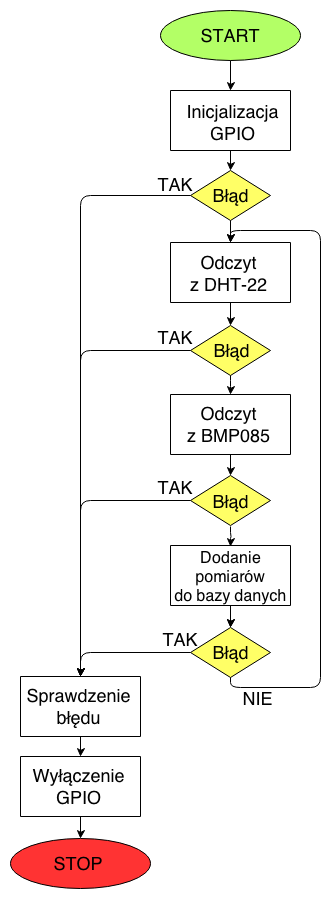
\includegraphics[scale=0.6]{diagram_program}
\caption{Diagram programu głównego stacji pogodowej}
\label{fig:diagram_program}
\end{figure}

\section*{Używanie MySQL z poziomu języka C}
Baza danych MySQL zostanie szerzej przedstawiona w następnym rozdziale.

Posiadając odebrane prawidłowe pomiary z czujników, należy je następnie zamieścić w bazie danych, aby były one dostępne do wyświetlania lub analizowania. W tym celu potrzebny jest sposób na umieszczenie danych do tej bazy z poziomu programu napisanego w języku C.

Producent bazy danych MySQL udostępnił interfejs komunikacyjny bazy, gotowy do zaimplementowania w C. Nazywa się on MySQL C API i jest dostępny dla wszyskich użytkowników za darmo. MySQL C API jest to biblioteka funkcji, która umożliwia komunikację programu z bazą danych MySQL.




